\chapter{Analiza wyników}


\section{Ocena jakości różnych architektur sieci neuronowych}

\begin{table}
    \caption{Podsumowanie miary F1 dla poszczególnych klas (EfficientNet B4)}
    \begin{center}
        \begin{tabular}{|l|l|l|l|l|}
            \hline
            Klasa & Precyzja & Czułość & F1    & Liczba próbek \\
            \hline
            BLA   & 0.780    & 0.840   & 0.810 & 2311          \\
            \hline
            EBO   & 0.940    & 0.960   & 0.950 & 5532          \\
            \hline
            EOS   & 0.980    & 0.980   & 0.980 & 1192          \\
            \hline
            LYT   & 0.910    & 0.930   & 0.920 & 5193          \\
            \hline
            MON   & 0.720    & 0.730   & 0.720 & 825           \\
            \hline
            MYB   & 0.780    & 0.660   & 0.710 & 1323          \\
            \hline
            NGB   & 0.780    & 0.790   & 0.790 & 1962          \\
            \hline
            NGS   & 0.930    & 0.930   & 0.930 & 5984          \\
            \hline
            PEB   & 0.780    & 0.650   & 0.710 & 552           \\
            \hline
            PLM   & 0.940    & 0.860   & 0.900 & 1466          \\
            \hline
            PMO   & 0.830    & 0.840   & 0.840 & 2429          \\
            \hline
        \end{tabular}
    \end{center}
    \label{tab:f1_summary}
\end{table}

Niniejszy projekt ma za zadanie porównać różne architektury splotowych sieci neuronowych i wskazać, która z nich daje najlepsze rezultaty.
Dla każdej architektury wskazano jej wielkość (ilość parametrów trenowalnych) oraz ważony wynik F1.
Większy wynik F1 informuje o lepszym zachowaniu modelu w rozpoznawaniu typów komórek.

Warto zauważyć, że często wielkość sieci neuronowej (liczba wag) nie jest liniowo zależna z jakością uzyskiwanych predykcji.
Dzieje się tak ze względu na to, że pojemność zachowania informacji nawet w mniejszej sieci jest wystarczająca, by móc rozpoznawać rodzaje komórek.

\begin{figure}
    \centering
    \includegraphics[width=\textwidth]{experiments/efficientnet_b0/combined}
    \caption{Wykres zależności funkcji straty i F1 od epoki trenowania (EfficientNet B0)}
    \label{fig:plot_efficientnet_b0}
\end{figure}
\begin{figure}
    \centering
    \includegraphics[width=0.8\textwidth]{experiments/efficientnet_b0/confusion_matrix}
    \caption{Macierz pomyłek modelu EfficientNet B0}
    \label{fig:confusion_efficientnet_b0}
\end{figure}

\begin{figure}
    \centering
    \includegraphics[width=\textwidth]{experiments/efficientnet_b1/combined}
    \caption{Wykres zależności funkcji straty i F1 od epoki trenowania (EfficientNet B1)}
    \label{fig:plot_efficientnet_b1}
\end{figure}
\begin{figure}
    \centering
    \includegraphics[width=0.8\textwidth]{experiments/efficientnet_b1/confusion_matrix}
    \caption{Macierz pomyłek modelu EfficientNet B1}
    \label{fig:confusion_efficientnet_b1}
\end{figure}

\begin{figure}
    \centering
    \includegraphics[width=\textwidth]{experiments/efficientnet_b2/combined}
    \caption{Wykres zależności funkcji straty i F1 od epoki trenowania (EfficientNet B2)}
    \label{fig:plot_efficientnet_b2}
\end{figure}
\begin{figure}
    \centering
    \includegraphics[width=0.8\textwidth]{experiments/efficientnet_b2/confusion_matrix}
    \caption{Macierz pomyłek modelu EfficientNet B2}
    \label{fig:confusion_efficientnet_b2}
\end{figure}

\begin{figure}
    \centering
    \includegraphics[width=\textwidth]{experiments/efficientnet_b3/combined}
    \caption{Wykres zależności funkcji straty i F1 od epoki trenowania (EfficientNet B3)}
    \label{fig:plot_efficientnet_b3}
\end{figure}
\begin{figure}
    \centering
    \includegraphics[width=0.8\textwidth]{experiments/efficientnet_b3/confusion_matrix}
    \caption{Macierz pomyłek modelu EfficientNet B3}
    \label{fig:confusion_efficientnet_b3}
\end{figure}

\begin{figure}
    \centering
    \includegraphics[width=\textwidth]{experiments/efficientnet_b4/combined}
    \caption{Wykres zależności funkcji straty i F1 od epoki trenowania (EfficientNet B4)}
    \label{fig:plot_efficientnet_b4}
\end{figure}
\begin{figure}
    \centering
    \includegraphics[width=0.8\textwidth]{experiments/efficientnet_b4/confusion_matrix}
    \caption{Macierz pomyłek modelu EfficientNet B4}
    \label{fig:confusion_efficientnet_b4}
\end{figure}

\begin{figure}
    \centering
    \includegraphics[width=\textwidth]{experiments/efficientnet_b5/combined}
    \caption{Wykres zależności funkcji straty i F1 od epoki trenowania (EfficientNet B5)}
    \label{fig:plot_efficientnet_b5}
\end{figure}
\begin{figure}
    \centering
    \includegraphics[width=0.8\textwidth]{experiments/efficientnet_b5/confusion_matrix}
    \caption{Macierz pomyłek modelu EfficientNet B5}
    \label{fig:confusion_efficientnet_b5}
\end{figure}

\begin{figure}
    \centering
    \includegraphics[width=\textwidth]{experiments/densenet121/combined}
    \caption{Wykres zależności funkcji straty i F1 od epoki trenowania (DenseNet121)}
    \label{fig:plot_densenet121}
\end{figure}
\begin{figure}
    \centering
    \includegraphics[width=0.8\textwidth]{experiments/densenet121/confusion_matrix}
    \caption{Macierz pomyłek modelu DenseNet121}
    \label{fig:confusion_densenet121}
\end{figure}

\begin{figure}
    \centering
    \includegraphics[width=\textwidth]{experiments/densenet169/combined}
    \caption{Wykres zależności funkcji straty i F1 od epoki trenowania (DenseNet169)}
    \label{fig:plot_densenet169}
\end{figure}
\begin{figure}
    \centering
    \includegraphics[width=0.8\textwidth]{experiments/densenet169/confusion_matrix}
    \caption{Macierz pomyłek modelu DenseNet169}
    \label{fig:confusion_densenet169}
\end{figure}

\begin{figure}
    \centering
    \includegraphics[width=\textwidth]{experiments/densenet201/combined}
    \caption{Wykres zależności funkcji straty i F1 od epoki trenowania (DenseNet201)}
    \label{fig:plot_densenet201}
\end{figure}
\begin{figure}
    \centering
    \includegraphics[width=0.8\textwidth]{experiments/densenet201/confusion_matrix}
    \caption{Macierz pomyłek modelu DenseNet201}
    \label{fig:confusion_densenet201}
\end{figure}

\begin{figure}
    \centering
    \includegraphics[width=\textwidth]{experiments/resnet18/combined}
    \caption{Wykres zależności funkcji straty i F1 od epoki trenowania (ResNet18)}
    \label{fig:plot_resnet18}
\end{figure}
\begin{figure}
    \centering
    \includegraphics[width=0.8\textwidth]{experiments/resnet18/confusion_matrix}
    \caption{Macierz pomyłek modelu ResNet18}
    \label{fig:confusion_resnet18}
\end{figure}

\begin{figure}
    \centering
    \includegraphics[width=\textwidth]{experiments/resnet50/combined}
    \caption{Wykres zależności funkcji straty i F1 od epoki trenowania (ResNet50)}
    \label{fig:plot_resnet50}
\end{figure}
\begin{figure}
    \centering
    \includegraphics[width=0.8\textwidth]{experiments/resnet50/confusion_matrix}
    \caption{Macierz pomyłek modelu ResNet50}
    \label{fig:confusion_resnet50}
\end{figure}

\begin{figure}
    \centering
    \includegraphics[width=\textwidth]{experiments/resnet101/combined}
    \caption{Wykres zależności funkcji straty i F1 od epoki trenowania (ResNet101)}
    \label{fig:plot_resnet101}
\end{figure}
\begin{figure}
    \centering
    \includegraphics[width=0.8\textwidth]{experiments/resnet101/confusion_matrix}
    \caption{Macierz pomyłek modelu ResNet101}
    \label{fig:confusion_resnet101}
\end{figure}

\begin{figure}
    \centering
    \includegraphics[width=\textwidth]{experiments/vgg16/combined}
    \caption{Wykres zależności funkcji straty i F1 od epoki trenowania (VGG16)}
    \label{fig:plot_vgg16}
\end{figure}
\begin{figure}
    \centering
    \includegraphics[width=0.8\textwidth]{experiments/vgg16/confusion_matrix}
    \caption{Macierz pomyłek modelu VGG16}
    \label{fig:confusion_vgg16}
\end{figure}

\begin{figure}
    \centering
    \includegraphics[width=\textwidth]{experiments/vgg19/combined}
    \caption{Wykres zależności funkcji straty i F1 od epoki trenowania (VGG19)}
    \label{fig:plot_vgg19}
\end{figure}
\begin{figure}
    \centering
    \includegraphics[width=0.8\textwidth]{experiments/vgg19/confusion_matrix}
    \caption{Macierz pomyłek modelu VGG19}
    \label{fig:confusion_vgg19}
\end{figure}

\begin{figure}
    \centering
    \includegraphics[width=\textwidth]{experiments/alexnet/combined}
    \caption{Wykres zależności funkcji straty i F1 od epoki trenowania (AlexNet)}
    \label{fig:plot_alexnet}
\end{figure}
\begin{figure}
    \centering
    \includegraphics[width=0.8\textwidth]{experiments/alexnet/confusion_matrix}
    \caption{Macierz pomyłek modelu AlexNet}
    \label{fig:confusion_alexnet}
\end{figure}

\subsection{EfficientNet B0}
\textit{Liczba parametrów: 5.3M}

\textit{Ważony wynik F1: 0.860}

Najmniejszy wariant architektury EfficientNet, zawierający tylko 5.3M parametrów, oferuje jakość predykcji na poziomie ważonego wyniku F1 równego 0.86.
Na podstawie wykresu 4.1 można stwierdzić, że już pierwsza epoka treningu sieci daje satysfakcjonujące rezultaty.
Kolejne dwie epoki jedynie nieznacznie poprawiają jakość modelu.
Najczęściej mylonymi klasami jest klasa NGB (Krwinka biała pałeczkowata) i NGS (Segmentowany neutrofil) - rys.~\ref{fig:confusion_efficientnet_b0}.

\subsection{EfficientNet B1}
\textit{Liczba parametrów: 7.8M}

\textit{Ważony wynik F1: 0.850}

Dla treningu wariantu B1 architektury EfficientNet zachodzi nieznaczne przetrenowanie.
Na podstawie wykresu F1 (wyk.~\ref{fig:plot_efficientnet_b1}) można zobaczyć, że trenowanie w trzeciej epoce jedynie pogarsza jakość predykcji.
Sieć często myli klasy PEB (Proerytroblast) z EBO (Erytroblast) i NGB (Krwinka biała pałeczkowata) z NGS (Segmentowany neutrofil) - rys. ~\ref{fig:confusion_efficientnet_b1}.

\subsection{EfficientNet B2}
\textit{Liczba parametrów: 9.2M}

\textit{Ważony wynik F1: 0.860}

Architektura EfficientNet B2 dostarcza dostatecznej jakości prognoz już w pierwszej epoce treningu.
Kolejne epoki jedynie nieznacznie poprawiają jakość modelu (wyk.~\ref{fig:plot_efficientnet_b2}).
Najczęściej mylonymi klasami są MYB (Mielocyt) i PMO (Promielocyt) - rys.~\ref{fig:confusion_efficientnet_b2}.

\subsection{EfficientNet B3}
\textit{Liczba parametrów: 12.0M}

\textit{Ważony wynik F1: 0.870}

Proces treningu EfficientNet B3 wygląda bardzo podobnie jak trening EfficientNet B2. Model natomiast charakteryzuje się nieco lepszą miarą F1 równą 0.87 w porównaniu do 0.86 modelu B2 (wyk.~\ref{fig:plot_efficientnet_b3}). Najczęściej mylonymi klasami są MYB (Mielocyt) i PMO (Promielocyt) oraz PEB (Proerytroblast) i EBO (Erytroblast) - rys.~\ref{fig:confusion_efficientnet_b3}.

\subsection{EfficientNet B4}
\textit{Liczba parametrów: 19.0M}

\textit{Ważony wynik F1: 0.880}

Jest to najlepszy model uzyskany w trakcie badań projektu inżynierskiego.
Jego wynik F1 wynosi 0.88 (wyk.~\ref{fig:plot_efficientnet_b4}). Najczęściej mylonymi klasami są MYB (Mielocyt) i PMO (Promielocyt) - rys.~\ref{fig:confusion_efficientnet_b4}.
Tabela ~\ref{tab:f1_summary} przedstawia zestawienie precyzji, czułości i F1 dla poszczególnych klas.

\subsection{EfficientNet B5}
\textit{Liczba parametrów: 30.0M}

\textit{Ważony wynik F1: 0.860}

Pomimo tego, że model ten zawiera więcej parametrów niż EfficientNet B4, miara F1 wynosi 0.86, co oznacza, że jego predykcje są gorsze niż w przypadku EfficientNet B4 (wyk.~\ref{fig:plot_efficientnet_b5}).
Najczęściej mylonymi klasami są MYB (Mielocyt) i PMO (Promielocyt) - rys.~\ref{fig:confusion_efficientnet_b5}.

\subsection{DenseNet121}
\textit{Liczba parametrów: 8.0M}

\textit{Ważony wynik F1: 0.850}

Architektura DenseNet121 trenuje się podobnie jak architektury EfficientNet - to znaczy już w pierwszej epoce treningu ważony wynik F1 jest bliski temu po trzeciej epoce (wyk.~\ref{fig:plot_densenet121}).
Najczęściej mylonymi klasami są NGB (Krwinka biała pałeczkowata) i NGS (Segmentowany neutrofil) oraz MYB (Mielocyt) i PMO (Promielocyt) - rys.~\ref{fig:confusion_densenet121}.

\subsection{DenseNet169}
\textit{Liczba parametrów: 14.1M}

\textit{Ważony wynik F1: 0.840}

Sieć głównie trenuje się w pierwszej epoce, dwie kolejne nieznacznie poprawiają jej jakość.
W trzeciej epoce widać oznaki nadmiernego dopasowania (wyk.~\ref{fig:plot_densenet169}).
Najczęściej mylonymi klasami są MON (Monocyt) i BLA (Blast) oraz MYB (Mielocyt) i PMO (Promielocyt) - rys.~\ref{fig:confusion_densenet169}.

\subsection{DenseNet201}
\textit{Liczba parametrów: 20.0M}

\textit{Ważony wynik F1: 0.850}

Przebieg treningu DenseNet201 przypomina trening DenseNet169.
Po trzeciej epoce nie występuje jednak nadmierne dopasowanie (wyk.~\ref{fig:plot_densenet201}), a najczęściej mylonymi klasami są MON (Monocyt) i BLA (Blast) oraz MYB (Mielocyt) i PMO (Promielocyt) - rys.~\ref{fig:confusion_densenet201}.

\subsection{ResNet18}
\textit{Liczba parametrów: 11.7M}

\textit{Ważony wynik F1: 0.840}

Architektura ResNet18, zawierając 11.7M parametrów, oferuje gorszą jakość predykcji (wyk.~\ref{fig:plot_resnet18}) niż przykładowo EfficientNet B2, która posiada 9.2M parametrów (ważony wynik F1 sieci ResNet wynosi 0.84 w porównaniu do 0.86 sieci EfficientNet B2).
Najczęściej mylonymi klasami są MYB (Mielocyt) i PMO (Promielocyt) - rys.~\ref{fig:confusion_resnet18}.

\subsection{ResNet50}
\textit{Liczba parametrów: 25.6M}
% TODO
\textit{Ważony wynik F1: 0.740}

\subsection{ResNet101}
\textit{Liczba parametrów: 44.7M}
% TODO
\textit{Ważony wynik F1: 0.770}

\subsection{VGG16}
\textit{Liczba parametrów: 138.4M}
% TODO
\textit{Ważony wynik F1: 0.070}

\subsection{VGG19}
\textit{Liczba parametrów: 143.7M}
% TODO
\textit{Ważony wynik F1: 0.070}


\subsection{AlexNet}
\textit{Liczba parametrów: 60M}
% TODO
\textit{Ważony wynik F1: 0.070}


\newline
\newline
\newline

%TODO net
Najlepsze wyniki uzyskuje model używający architektury \textit{EfficientNet B4}.
Ważony wynik F1 w jej przypadku wynosi \textit{0.88}.

Na podstawie wykresów funkcji straty i F1, można stwierdzić, że dla wszystkich sieci neuronowych już pierwsza epoka skutkowała rozpoznaniem wzorców.
Kolejne epoki nie poprawiały znacząco skuteczności sieci.
Często mylonymi komórkami były promielocyty (\textit{PMO}) i mielocyty (\textit{MYB}), wynika to z tego, że ich wygląd jest podobny.


\section{Porównanie z innymi algorytmami}

\begin{figure}
    \centering
    \includegraphics[width=0.6\textwidth]{images/resnext_confusion_matrix}
    \caption{Macierz pomyłek dla modelu ResNeXt \cite{resnext}}
    \label{fig:resnext_confusion_matrix}
\end{figure}

Dostawca zbioru danych, w artykule \textit{Highly accurate differentiation of bone marrow cell morphologies using deep neural networks on a large image dataset}~\cite{resnext} wykorzystuje architekturę \textit{ResNetXt-50}.
Model zawierający ponad 23 miliony parametrów był trenowany na \textit{NVIDIA TESLA V100} przez ok. 48 godzin.
Podobnie jak w niniejszym projekcie, autorzy artykułu wykonali normalizację intensywności kolorów przed trenowaniem sieci neuronowej (z powodu różnic w barwieniu Maya-Grünwalda-Giemsa).
Uzyskany ważony wynik F1 dla architektury \textit{ResNeXt-50} wyniósł \textit{0.822}.
Macierz pomyłek dostarczona przed autorów pracy jest widoczna na rys. \ref{fig:resnext_confusion_matrix}.


\section{Wyzwania}

Głównym wyzwaniem w trakcie realizacji projektu było wytrenowanie dużych sieci neuronowych.
Niestety, ich trening na lokalnym sprzęcie takim jak komputer osobisty jest bardzo czasochłonny.
W związku z tym konieczne było uruchamianie ich na platformie \textit{kaggle.com}, która oferuje 30 godzin czasu procesora graficznego miesięcznie.
Nieodpłatna możliwość pracy na platformie pozwoliła na pomyślną realizację projektu.


\section{Wnioski}

%TODO net
Zaprezentowane porównanie różnych splotowych sieci neuronowych pokazuje, że najlepszym modelem do zadania klasyfikacji rodzajów komórek w szpiku kostnym jest \textit{EfficientNet B4}.
Wybrana sieć neuronowa uzyskuje najlepszy ważony wynik F1 równy \textit{0.88}.
Warto też zwrócić uwagę na to, że sieci neuronowe znacznie większe od \textit{EfficientNet B4} nie dawały dużo lepszych rezultatów.

